
\begin{figure}
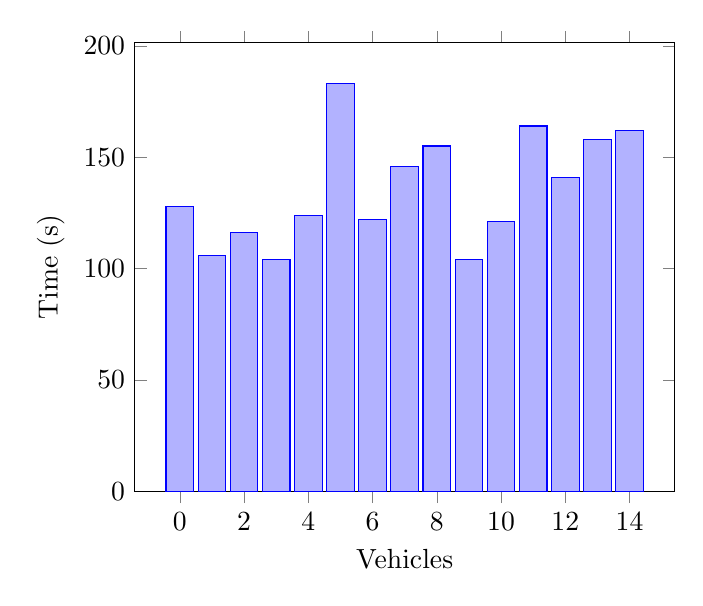
\begin{tikzpicture}
\begin{axis}[
legend style={anchor=west},
xlabel=Vehicles,
ylabel=Time (s),
ymin=0,
ybar,
]
\addplot coordinates {
(0, 128)
(1, 106)
(2, 116)
(3, 104)
(4, 124)
(5, 183)
(6, 122)
(7, 146)
(8, 155)
(9, 104)
(10, 121)
(11, 164)
(12, 141)
(13, 158)
(14, 162)
};

\end{axis}
\end{tikzpicture}
\label{tik:100:19_O, 19_O.-60, 17_N, 15_S, 15_S.-30, 13_N, 13_N.-40, 11_N, 8_N, 7_N, 7_N.-60, 5_N, 4_N, 4_N.-60, 2_V}
\caption{100 percent diving with GSC on route $19_O, 19_O.-60, 17_N, 15_S, 15_S.-30, 13_N, 13_N.-40, 11_N, 8_N, 7_N, 7_N.-60, 5_N, 4_N, 4_N.-60, 2_V$}
\end{figure}
